\documentclass[pdftex,12pt,letter]{article}
\usepackage[binary-units=true]{siunitx}
\usepackage[margin=0.75in]{geometry}
\usepackage[utf8]{inputenc}
\usepackage[T1]{fontenc}
\usepackage{graphicx}
\usepackage{amsmath}
\usepackage{xspace}
\usepackage{xcolor}
\usepackage[pdftex,pdfpagelabels,bookmarks,hyperindex,hyperfigures]{hyperref}

\newcommand{\fixme}[1]{\textcolor{red}{\textit{Fixme}: \textbf{#1}}}


\author{Brett Viren}
\date{\today (draft)}
\title{Single-Phase protoDUNE TPC Numbers}
\begin{document}

\maketitle

\begin{abstract}
The numbering used for the single-phase protoDUNE TPC is described.
\end{abstract}


\section{Overview}

This document describes the numbers involved in labeling parts of the
single-phase protoDUNE detector related to the TPC.  The document is
ordered in the direction of information flow starting from ionization
activity in the liquid argon and ending with raw data on disk.  For
each stage stage of this flow, a numbering convention is
proposed\footnote{While this document is in draft, expect these
  conventions to change as we settle on a global optimum.}.  Other
known, relevant conventions which differ are given for reference and
to facilitate mappping.

A global orientation is adopted which takes approximate direction from
the expected particle beam.  This is taken from conventions developed
by the installation group and shown in table~\ref{tab:global}.

\begin{table}[htp]
  \label{tab:global}
  \centering
  \begin{tabular}[h]{|c|c|c|}
    \hline
    \multicolumn{3}{|c|}{North aka Beam Left} \\
    \hline
    Upstream & Midstream & Downstream \\
    \hline
    \multicolumn{3}{|c|}{South aka Beam Right} \\
    \hline
    \multicolumn{3}{c}{$\longrightarrow$ approximate beam direction $\longrightarrow$} \\    
  \end{tabular}
  \caption{Global orientation labels.  Beam travels approximately left to
    right.  Up-, mid- and down-stream may be abbreviated US, MS and
    DS, respectively.  Beam-left (BL) and beam-right (BR) are on the
    North and South sides of the detector, respectively}
\end{table}

In the following sections each part of the detector is described and
numbered w.r.t. the part the ``contains'' it.  That is, they represent
\textit{local numbering} which is assumed to replicate for as-designed
numbering following the symmetry of the detector.  Any as-built
deviations will need to be handled.  Following the sections describing
local numbering is one describing a scheme to generate \textit{global
  numbering} from the ensemble of local numbers.


\section{TPC Drift Cells}

The TPC has 6 ``large'' or ``central'' drift cells full of liquid
argon bounded by a face of a CPA and an APA.  The opposite face of the
APA is sensitive to activity that occurs in another ``thin'' or
``edge'' drift cell giving a total of 12 drift cells.

It is not expected that the raw data will contain TPC drift cell
numbers, per se.  However, there is a one-to-one correlation between
and APA face and a TPC drift cell.  The drift cell number is most
important for offline simulation and reconstruction where, for
example, one must label portions of activity of interaction that span
multiple cells.

Current LArSoft TPC numbering rasters a count in ``drift-major''
ordering irrespective of the difference between edge and central TPCs.
See table~\ref{tab:lstpc}.

As that numbering does not give precedence to the most interesting,
central TPCs an alternative is proposed here for adoption as official
convention and with hopes that it is implemented in the next version
of LArSoft.  To produce synergy with installation numbering the
central TPCs are numbered by the installation numbers for the APAs
(see table~\ref{tab:installapa}) which (partially) view them.  The
``edge'' TPC cells are further counted in the same order.  This allows
the numbers for the TPC drift cells on either side of an APA to differ
by a fixed value of six.

Note, there is no TPC 0 due to aligning with installation APA numbers.
This has a beneficial side effect as allowing TPC number 0 to indicate
error or other exceptional condition in the offline software.  It does
mean that an APA number can not directly be used as an index into an
array but simply must have unity subtracted.


\begin{table}[htp]
  \label{tab:tpc}
  \centering
  \begin{tabular}[h]{|c|c|c|}
    \hline\hline
    12 & 11 & 10\\
    \hline
    \hline
    \multicolumn{3}{|c|}{APAs}\\
    \hline
    \hline
    6 & 5 & 4 \\
    \hline
    \hline
    \multicolumn{3}{|c|}{CPAs}\\
    \hline
    \hline
    3 & 2 & 1 \\
    \hline
    \hline
    \multicolumn{3}{|c|}{APAs}\\
    \hline
    \hline
    9 & 8 & 7 \\
    \hline
    \hline
    \multicolumn{3}{c}{beam $\longrightarrow$} \\    

  \end{tabular}
  \caption{Proposed TPC drift cell numbering convention which is based
    on the convention used by the installation group for the APA
    counts}
\end{table}



\begin{table}[htp]
  \label{tab:lstpc}
  \centering
  \begin{tabular}[h]{|c|c|c|}
    \hline\hline
    3 & 7 & 11\\
    \hline
    \hline
    \multicolumn{3}{|c|}{APAs}\\
    \hline
    \hline
    2 & 6 & 10 \\
    \hline
    \hline
    \multicolumn{3}{|c|}{CPAs}\\
    \hline
    \hline
    1 & 5 & 9 \\
    \hline
    \hline
    \multicolumn{3}{|c|}{APAs}\\
    \hline
    \hline
    0 & 4 & 8 \\
    \hline
    \hline
    \multicolumn{3}{c}{beam $\longrightarrow$} \\    
  \end{tabular}
  \caption{Current LArSoft TPC numbering taken from dunetpc wiki~\cite{dunetpc-wiki}.  These are not proposed for convention. \fixme{Check is beam direction/number correlation is correct.}}
\end{table}


\section{APA}

\fixme{This is my current understanding, need checking from cold
  electronics, WIB and DAQ experts.}  Each APA is an independent data
source for the artDAQ based DAQ.  It is the ``Board Reader'' node of
the DAQ which assigns APA number.  The APA numbering convention
asserted here for the DAQ to follow matches the installation numbering
convention and is described in table~\ref{tab:apa}.

\begin{table}[htp]
  \label{tab:apa}
  \centering
  \begin{tabular}[h]{|c|c|c|}
    \hline
    6 & 5 & 4 \\
    \hline
    \hline
    3 & 2 & 1 \\
    \hline
    \hline
    \multicolumn{3}{c}{beam $\longrightarrow$} \\    

  \end{tabular}
  \caption{Proposed APA numbering numbering convention which matches that used by the installation group.}
\end{table}


\section{APA Faces}

Each APA has two faces.  The face continuing wires which are sensitive
to activity in the ``central'' drift cell may be referred to as the
``main'' or ``inner'' face and takes a face number 0.  The ``other''
or ``edge'' face takes number 1.  This is illustrated in
table~\ref{tab:faces}.


\begin{table}[htp]
  \label{tab:apa}
  \centering
  \begin{tabular}[h]{|c|}
    \hline
    edge drift cell\\
    \hline
    \hline
    outer face: 1\\
    \hline
    APA frame\\
    \hline
    inner face: 0 \\
    \hline
    \hline
    central drift cell \\
    \hline
    \multicolumn{1}{c}{beam $\longrightarrow$} \\

  \end{tabular}
  \caption{APA face numbering, drawn for a beam-left APA.  A
    180$^\circ$ rotation is applied to describe APAs on the beam-right
    side of the detector.}
\end{table}


\section{Wires}

A wire \textit{conductor} is an electrically contiguous run of
conducting material which feeds in to one electronics channel.  Where
a conductor spans an APA face along a straight line it is called a
wire \textit{segment} or just \textit{wire}.

The wires for one face of one APA are shown in Figure~\ref{fig:wires}.
Only one in twenty wires are shown.

\section{Segment in a conductor}

Because the conductors that contribute to ``induction'' wire planes
wrap around the APA they may have up to three wire segments while the
conductors which make up a ``collection'' wire plane have a single
segment.  These segments are counted starting from zero at the point
where they attach to the \textit{wire boards} at the top of an APA
face.  The segment number is indicated by the thickness of the line in
Figure~\ref{fig:wires}.  

\begin{figure}[htp]
  \centering
  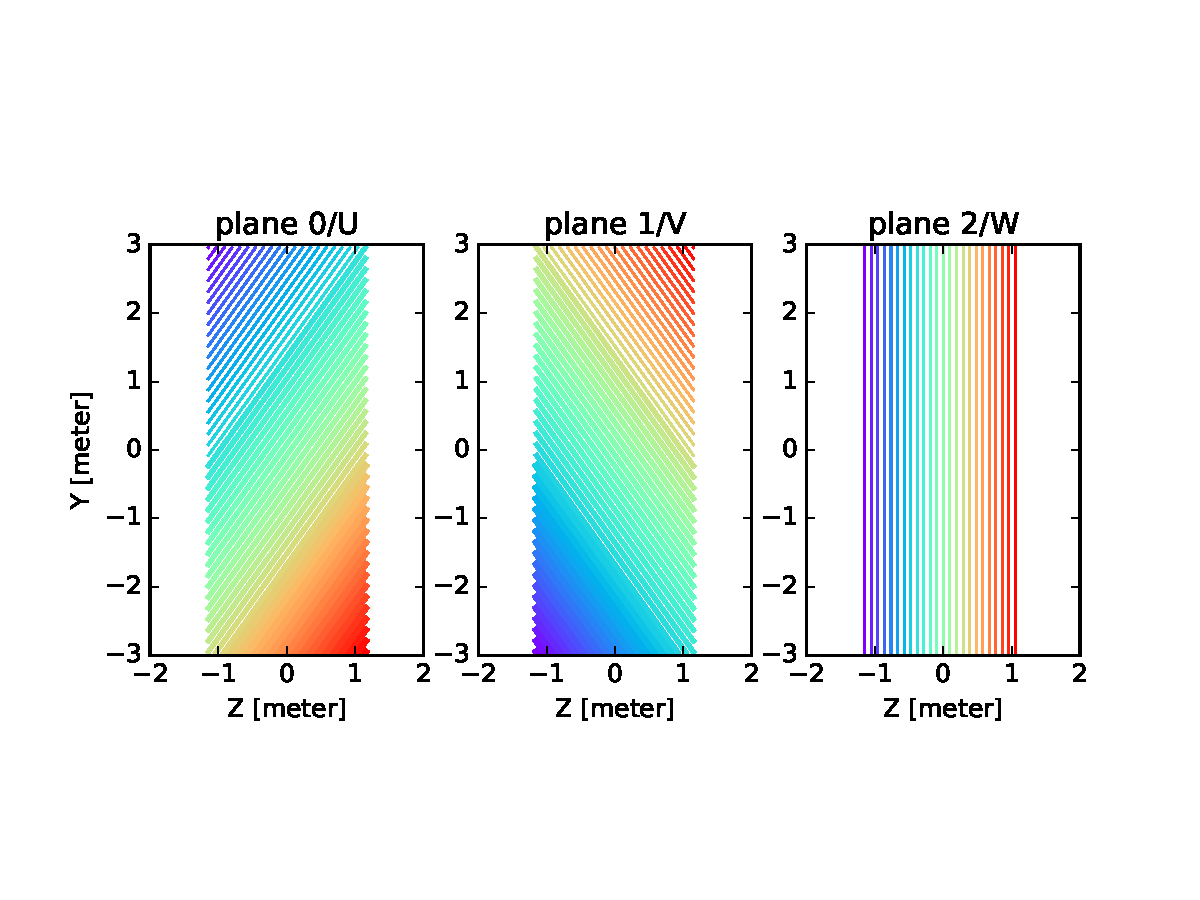
\includegraphics[width=\textwidth]{wires-20.pdf}
  \caption{The wire (segments) for each wire plane on one face of one APA for protoDUNE.  Increasing width of the wire indicates increasing segment number (0, 1 or 2) and the color indicates increasing wire number from blue to red.  Only one of every twenty wires are shown. The Y coordinate points opposite of gravity.  The unlabeled X coordinate is into the page and is counter to the drift direction.  Z follows from the right-hand-rule.  \fixme{Check that U/V directions are correct.}}
  \label{fig:wires}
\end{figure}

\section{Wires in a plane.}

Wires in one plane provide a local orthogonal Cartesian coordinate
system that is useful for simulation and reconstruction.  The basis of
this coordinate system is composed of unit vectors in the following
directions, in order:

\begin{description}
\item[$v_1 \equiv v_d$] The anti-drift direction, which is same as the positive X direction local to the drift cell.
\item[$v_2 \equiv v_w$] The direction along the wire toward the input to the electronics.
\item[$v_3 \equiv v_p$] The direction along the wire pitch.
\end{description}

These are ordered such that the right-handed cross product
$v_d \times v_w = v_p$ holds.  A rotation transform relates this basis
with one associated with another orthogonal coordinate system attached
to the local drift cell.  Each wire plane coordinate system (for a
given APA face) shares the X direction ($v_d$) with the local drift
cell coordinate system.  The Y coordinate points counter to gravity
and Z follows from the right hand rule.

Teh pitch position of a wire increases generally as Z increases.  In
Figure~\ref{fig:wires} pitch increases as the color transitions from
blue to red.

When ordered by pitch, the wires in a plane are given an index.  This
\textit{wire pitch index} counts starting from 0 at the smallest pitch
(most negative Z).

\section{Wire attachment numbers}

All segment-0 wires in a given plane on one face of one APA attach to
ten \textit{wire boards} mounted at the top of the APA frame.  Their
\textit{wire attachment points} for each plane form an ordered and
regular line.  In order to match the local numbering convention of the
electronics (next sections) the \textit{wire attachment numbers} count
start from 1 and advance as one goes left-to-right facing the APA.
This means that they increase with decreasing Z.  Note: the wire
attachment numbering starts counting from 1 to match the convention
used by the electronics. \fixme{The ordering with Z here is from decoding
  drawings and may be swapped!  If so, the numbering directions that
  follow the WAN numbering also need swapping.}

\begin{table}[htp]
  \centering
  \begin{tabular}[h]{ccc}
    \hline
    2/U & 400 & 1 \\
    \hline
    1/V & 400 & 1 \\
    \hline
    0/W & 480 & 1 \\
    \hline
    outer face & $Z<0$  & $Z>0$\\
    \hline
    \multicolumn{3}{|c|}{APA frame}\\
    \hline
    inner face & $Z>0$ & $Z<0$\\
    \hline
    0/W & 1 & 480 \\
    \hline
    1/V & 1 & 400 \\
    \hline
    2/U & 1 & 400 \\
    \hline
  \end{tabular}
  \caption{Illustration of wire attachement numbers for one APA.  Each wire plane attaches in a line of points at the top of the APA.  These points are counted starting from 1 to match electronics convention and increase as one decreases in the local Z coordinate.  The numbering is $180^\circ$ rotationally symmetric.}
  \label{tab:wan}
\end{table}

\section{Cold Electronics}

Each wire segment zero attaches to a \textit{wire board}.  There are
ten wire boards per each APA face.  These are numbered in the same
direction as the wire attachment numbers as shown in table~\ref{tab:wireboards}

\begin{table}[htp]
  \label{tab:wireboards}
  \centering
  \begin{tabular}[h]{ccc}
    \hline
     9 & -- & 0 \\
    \hline
    outer face & $Z<0$  & $Z>0$\\
    \hline
    \multicolumn{3}{|c|}{APA frame}\\
    \hline
    inner face & $Z>0$ & $Z<0$\\
    \hline
    0 & -- & 9 \\
    \hline
  \end{tabular}
  \caption{Wire board numbering.}
\end{table}

Each wire board has attached input wires from all four wire planes
(including grid plane) and locally numbered as shown in
table~\ref{tab:wireboard} matching reference~\cite{docdb2060-v3-adaptor-board-0}.

\begin{table}[htp]
  \label{tab:wireboard}
  \centering
  \begin{tabular}[h]{ccc}
    plane & label & numbering \\
    3 & G & 1 -- 48 \\
    2 & W & 1 -- 48 \\
    1 & V & 1 -- 40 \\
    0 & U & 1 -- 40 \\
  \end{tabular}
  \caption{Local wire board wire attachment numbering.  Numbers increase in the same direction as wire attachment numbering which is in decreasing Z.}
\end{table}

Each wire board has associated a front-end motherboard (FEMB) with
eight FEE amplifier and ADC ASIC pairs numbered 1-8.  Each pair of
ASICs has 16 channels numbered 0-15.  The mapping from local wire
board attachment number to ASIC and local ASIC channel numbers
involves a nontrivial map.  This map is exhaustively given in
reference~\cite{wirechmap} and reproduced in a matrix form in
table~\ref{tab:wirechmap}.

This association between the numbers of an ASIC and its channel with a
local wire board wire identifier repeats ten times as one goes down
one top face of an APA.  This per-face pattern repeats on the opposite
face, obeying a $180^\circ$ rotational symmetry.

\begin{table}[htp]
  \label{tab:wirechmap}
  \centering
% Note: this table can be generated using chmap.py.

\begin{tabular}{r|rrrrrrrr}
\hline
ASIC:&1&2&3&4&5&6&7&8\\
\hline
ch00 & \textcolor{red}{u19} & \textcolor{red}{u09} & \textcolor{black}{w14} & \textcolor{black}{w02} & \textcolor{red}{u29} & \textcolor{red}{u39} & \textcolor{black}{w26} & \textcolor{black}{w38}\\
ch01 & \textcolor{red}{u17} & \textcolor{red}{u07} & \textcolor{black}{w16} & \textcolor{black}{w04} & \textcolor{red}{u27} & \textcolor{red}{u37} & \textcolor{black}{w28} & \textcolor{black}{w40}\\
ch02 & \textcolor{red}{u15} & \textcolor{red}{u05} & \textcolor{black}{w18} & \textcolor{black}{w06} & \textcolor{red}{u25} & \textcolor{red}{u35} & \textcolor{black}{w30} & \textcolor{black}{w42}\\
ch03 & \textcolor{red}{u13} & \textcolor{red}{u03} & \textcolor{black}{w20} & \textcolor{black}{w08} & \textcolor{red}{u23} & \textcolor{red}{u33} & \textcolor{black}{w32} & \textcolor{black}{w44}\\
ch04 & \textcolor{red}{u11} & \textcolor{red}{u01} & \textcolor{black}{w22} & \textcolor{black}{w10} & \textcolor{red}{u21} & \textcolor{red}{u31} & \textcolor{black}{w34} & \textcolor{black}{w46}\\
ch05 & \textcolor{blue}{v19} & \textcolor{blue}{v09} & \textcolor{black}{w24} & \textcolor{black}{w12} & \textcolor{blue}{v29} & \textcolor{blue}{v39} & \textcolor{black}{w36} & \textcolor{black}{w48}\\
ch06 & \textcolor{blue}{v17} & \textcolor{blue}{v07} & \textcolor{blue}{v12} & \textcolor{blue}{v02} & \textcolor{blue}{v27} & \textcolor{blue}{v37} & \textcolor{blue}{v22} & \textcolor{blue}{v32}\\
ch07 & \textcolor{blue}{v15} & \textcolor{blue}{v05} & \textcolor{blue}{v14} & \textcolor{blue}{v04} & \textcolor{blue}{v25} & \textcolor{blue}{v35} & \textcolor{blue}{v24} & \textcolor{blue}{v34}\\
ch08 & \textcolor{blue}{v13} & \textcolor{blue}{v03} & \textcolor{blue}{v16} & \textcolor{blue}{v06} & \textcolor{blue}{v23} & \textcolor{blue}{v33} & \textcolor{blue}{v26} & \textcolor{blue}{v36}\\
ch09 & \textcolor{blue}{v11} & \textcolor{blue}{v01} & \textcolor{blue}{v18} & \textcolor{blue}{v08} & \textcolor{blue}{v21} & \textcolor{blue}{v31} & \textcolor{blue}{v28} & \textcolor{blue}{v38}\\
ch10 & \textcolor{black}{w23} & \textcolor{black}{w11} & \textcolor{blue}{v20} & \textcolor{blue}{v10} & \textcolor{black}{w35} & \textcolor{black}{w47} & \textcolor{blue}{v30} & \textcolor{blue}{v40}\\
ch11 & \textcolor{black}{w21} & \textcolor{black}{w09} & \textcolor{red}{u12} & \textcolor{red}{u02} & \textcolor{black}{w33} & \textcolor{black}{w45} & \textcolor{red}{u22} & \textcolor{red}{u32}\\
ch12 & \textcolor{black}{w19} & \textcolor{black}{w07} & \textcolor{red}{u14} & \textcolor{red}{u04} & \textcolor{black}{w31} & \textcolor{black}{w43} & \textcolor{red}{u24} & \textcolor{red}{u34}\\
ch13 & \textcolor{black}{w17} & \textcolor{black}{w05} & \textcolor{red}{u16} & \textcolor{red}{u06} & \textcolor{black}{w29} & \textcolor{black}{w41} & \textcolor{red}{u26} & \textcolor{red}{u36}\\
ch14 & \textcolor{black}{w15} & \textcolor{black}{w03} & \textcolor{red}{u18} & \textcolor{red}{u08} & \textcolor{black}{w27} & \textcolor{black}{w39} & \textcolor{red}{u28} & \textcolor{red}{u38}\\
ch15 & \textcolor{black}{w13} & \textcolor{black}{w01} & \textcolor{red}{u20} & \textcolor{red}{u10} & \textcolor{black}{w25} & \textcolor{black}{w37} & \textcolor{red}{u30} & \textcolor{red}{u40}\\
\hline
\end{tabular}


  \caption{Map between local wire board numbers and ADC and their channel numbers with U plane wires in \textcolor{red}{red} and V plane wires in \textcolor{blue}{blue}.  This single FEMB contains 128 wires, 40 in U and V planes and 48 in W.  This pattern of connectivity repeats 10 times down the top of the APA frame.}
\end{table}

\section{Warm Interface Boards}

The data from the 20 FEMBs reading out both faces of one APA feed into
five warm interface boards (WIB).

\fixme{What is the connection map here?}

\fixme{Where and in what manner does an FEMB get numbered?  Is it indeed the WIB that stamps one FEMB's data with an FEMB number?}

\fixme{Does a WIB know which WIB it is?}

\section{RCE and FELIX}

\fixme{There are two RCEs per APA.  How do they read out 5 WIBs?}

\fixme{Where and in what manner does an APA get numbered?}

\section{Global Numbering}

The numbering conventions above are all local to a unique unit of the
detector.  As such a collection of different numbers are needed to
uniquely identify the smallest units.  With some redundancy, the list
of quantities that can be specified are summarized from the above
sections as:

\begin{itemize}
\item $G_{tpc}$ global TPC number (central: 1-6 and edge: 7-12)
\item $G_{apa}$ global APA number (1-6)
\item $L_{face}$ local APA face (0,1)
\item $L_{wib}$ local WIB number (5, numbered like ??)
\item $L_{femb}$ local FEMB number on one face (1-10)
\item $L_{asic}$ local ASIC (pair, either FEE amp or ADC) on FEMB (1-8)
\item $L_{ch}$ local channel on ASIC (0-15)
\item $L_{plane}$ local wire plane holding (0/U, 1/V, 2/W).
\item $L_{seg}$ local wire segment number in conductor (W always 0, U/V $\in$ 0,1,2)
\item $L_{pitch}$ local wire pitch index in plane
\item $L_{wan}$ local wire attachment number on face of APA (U/V:1-400, W:1-480)
\end{itemize}

The mapping between these numbers are very ``shuffled'' due to wire
wrapping, ASIC-wire channel map, multiple APAs and the dichotomy of
``inner'' and ``outer'' faces.  There are also multiple levels in this
map which are interesting to access.  As such there is clearly no
ideal transformation to produce some a single global number suitable
for all parts.  Any choice for such a global number will be unsuitable
for some subset of use cases.  Forcing this choice is not a good
strategy.

Rather, a family of global numbering conventions is proposed.  In a
top-down order one obvious flattening presents itself:

\[  G_{face} = 1 + (G_{apa}-1) + 2\times L_{face} = G_{tpc} \in (1-12) \]
  
\[  G_{femb} = L_{femb} + 10\times (G_{face}-1) \in (1,120) \]

\[  G_{asic} = L_{asic} + 8\times (G_{femb}-1) \in (1,960) \]

\[ G_{ch} = L_{ch} + 16\times (G_{asic}-1) \in (0,15369) \]

Plots produced in terms of any of the above levels of granularity can
illustrate any effects which are localized to the corresponding
electronics unit.  However, effects that are localized in terms of
wires will not show well in such electronics units due to the
shuffling given in table~\ref{tab:wirechmap}.  A global wire
attachment number $L_{wan}$ can be constructed similarly to $G_{ch}$.

\fixme{Type out $L_{wan}$.}

\section{What else?}

t.b.d.






\end{document}

%%% Local Variables:
%%% mode: latex
%%% TeX-master: t
%%% End:
